\section{Introduction and Motivation}
The goal of this part of the project was to see whether a well known ferroelectric polymer could be used to enhance the efficiency of solar cell when applied as a thin film to its surface.\\
Solar cells convert light energy directly into electrical energy via the photoelectric effect and thus they are a proven method for obtaining sustainable energy. Significant amounts of research effort are put into exploring new materials and their possibilities as well as into improving existing types of solar cells. REF Broadly, one can divide the research approaches of solar energy conversion into two main categories: either a high quality, high cost approach that tries to maximise ultimate efficiencies as much as possible or a \enhyphen{low} quality, low cost approach that tries to strike an advantageous balance between production costs and obtained efficiency. The former is, for example, represented by complex III-IV multi-junction solar cells that maximise the usage of the available solar spectrum in each of their layers separately. REF Efficiencies as high as XXX\SI{0}{\percent} have been reported REF and even higher efficiencies may be reached when utilising light-concentrator schemes~\footnote{An added advantage of concentrators is that they allow collection of light over a great area with relatively cheap lens materials and minimise the area necessary for the costly actual cell.} REF. The second approach focuses more on new materials or tries to combine the advantages of wet-chemical production processes, namely their versatility and low cost, with solar cell preparation. Here, the Cahen group has made significant advances by showing how molecular surface modifications can be used to improve the efficiency of existing cells and by demonstrating a silicon inversion-layer type solar cell where the inversion layer is created by, again, molecular surface modifications REF. To explain a little further: in a \enhyphen{typical} silicon solar cell a p-n-junction is created by changing the type of dopant introduced into molten silicon during cell growth. This process is relatively costly in terms of energy and, accordingly, in terms of money as well. In an inversion-layer type solar cell, on the other hand, only one type of material (either p- or n-type doped silicon) is used and the necessary junction is formed by excluding one type of charge carriers in a thin layer directly the cell surface by a strong electric field created by chemisorbed dipolar molecules. In this respect, the attempt at creating a comparable effect by a physisorbed ferroelectric polymer is a logical continuation of ongoing work in the Cahen group. Furthermore, one significant loss mechanism in solar cells is unwanted surface recombination of created charge carriers. The efficiency of this loss mechanism is dependent on the product of the two types of charge carriers and therefore, if one type of charge carrier can be excluded from the surface, a reduction of losses is expected. Similar approaches are realised by, for example, including a back-surface field (\bfs{}) in industrially grown silicon solar cells REF. The ferroelectric polymer of choice has also been implemented as a \enhyphen{sandwich} layer in organic solar cells and was shown to increase efficiency REF, but some discussion about the mechanism by which this improvement is achieved still exists in the literature REF.\\
Having established why the combination of ferroelectric polymer with silicon solar cells may be of potential societal benefit and research interest, the polymer material will be introduced in detail in the following Section. In Section \ref{sec:exptech} the diverse experimental methods used throughout this project are introduced from a theoretical standpoint and in Section \ref{sec:expwork} the experimental approach is outlined and the obtained results are reported and discussed. The concluding Section gives a short summary of this part of the project and tries to analyse its failures as well as partial successes.

\section{\pvdf{}} 

\section{Experimental Techniques}
\label{sec:exptech}
\subsection{Contact Potential Difference and Surface Photovoltage}
Chapter \ref{chap:spv} deals exclusively with the contact potential difference (\cpd{}) and the surface photovoltage (\spv{}), so any theoretical or practical explanation will be skipped here.\\
For the scope of this Chapter, it is sufficient to mention that \cpd{} measures the work function of a sample compared to a known reference and that \spv{} can be an indicator of charges trapped at the surface and the overall quality of a chemical or physical surface modification. Previous work carried out at the Cahen group often focused on chemical surface modifications of silicon and it was shown for a range of chemicals that a (surface) dipole can influence the work function of the underlying silicon substrate. It is therefore assumed that successfully adsorbed \pvdf{} should influence the work function of silicon as measured by \cpd{} and that the direction of this influence be tune-able by changing the polarisation-direction of the ferroelectric polymer. It is furthermore assumed that a change in \spv{} may be taken as an indication of either less surface recombination or the presence of an electrical field at the surface.

\subsection{Determination of Excess Carrier Lifetimes}
In semiconductors, photogenerated excess charge carriers may recombine via different mechanisms. The effects of each of these mechanisms can be described by individual recombination rates, $S$ or by individual characteristic recombination \enhyphen{lifetimes}, $\tau$. Generally, a distinction has to be made between recombination in the bulk as expressed by the bulk carrier lifetime \tbulk{} and recombination at surfaces as expressed by the surface lifetime \tsurf{}. These two lifetimes combine to an effective carrier lifetime \teff{} given by:
\begin{equation}
\label{efflifetime}
	\frac{1}{\teff} = \frac{1}{\tbulk} + \frac{1}{\tsurf} \, .
\end{equation}
For the bulk, three mechanism can be identified: radiative recombination (also known as band-to-band recombination), \trad{}, where carriers of opposite charge neutralise each other and emit a photon of corresponding energy; Shockley-Read-Hall recombination , \tsrh{}, where carriers recombine via traps within the bandgap and Auger recombination, \taug{}, where opposite carriers recombine and transfer their energy to a third carrier, which subsequently gives off its excess energy in the form of heat. In the presence of these mechanisms, \tbulk{}, is given by:
\begin{equation}
\label{bulklifetime}
	\frac{1}{\tbulk} = \frac{1}{\trad} + \frac{1}{\tsrh} + \frac{1}{\taug} \, .
\end{equation}
For indirect bandgap semiconductors such as silicon, \trad{} is typically large compared to the other times and may be neglected in Equation \eqref{bulklifetime}. Conversely, for (high quality) direct bandgap semiconductors such as GaAs, \trad{} is short and \tsrh{} is typically large and may often be neglected~\cite{gaaslifetime}. Because Auger recombination is a three-particle process, it is inherently less probable than its two-particle counterparts. However, the Auger recombination rate is a cubic function of excess carrier density and therefore becomes dominant at higher carrier concentrations~\cite{auger}. Surfaces are natural defects in the crystal structure and as such provide ample opportunity for carriers to recombine. It is more difficult to generally relate the surface recombination velocities \ssurf{} to a surface recombination lifetime which can be used in Equation \eqref{efflifetime}. For example, the two large surfaces of a wafer might have different recombination velocities and in very high quality semiconductors, even the comparatively small surfaces at the edges may influence the overall effective lifetime~\cite{edgerecom}.\\
One method to measure the effective lifetime of the excess carriers of a semiconductor is to convert its photoconductance into its excess carrier density via known mobility functions:
\begin{equation}
\label{carrierbalance}
	\Delta n = \frac{\Delta \sigma}{qW (\mu_n \mu_p)} \, ,
\end{equation}
where $\sigma$ is the conductance, $\Delta n$ denotes the excess carrier density, $W$ is the sample thickness, $q$ the charge and $\mu_n$ \& $\mu_p$ are the mobilities of negative and positive carriers respectively. The situation is complicated because the mobilities generally are functions of the doping densities and also of the excess carrier density~\cite{sintononline}. Therefore, some knowledge about the sample is required and modelling the characteristics of the sample is generally applied. The carrier concentration in Equation \eqref{carrierbalance} can be converted to lifetimes by solving the continuity equations to obtain:
\begin{equation}
\label{taugeneral}
	\teff (\Delta n) = \frac{\Delta n (t)}{G(t) - \frac{d\Delta n}{dt} } \, ,
\end{equation}
in which $G(t)$ is the photogeneration rate and $\Delta n$ is, again, the excess carrier density~\cite{nagel_lifetime}. Equation \eqref{taugeneral} is generally valid and was even derived for non-uniform photogeneration in the presence of significant surface recombination. Most measurements are realised by flashing a strong light on the sample and monitoring the time-evolution of its photoconductance via a radio-frequency bridge. When the duration of the flash is long, a quasi-steady state situation is achieved in which the excess carrier density can be seen as constant in time. Equation \eqref{taugeneral} simplifies to:
\begin{equation}
\label{qsspd}
	\teff (\Delta n) = \frac{\Delta n (t)}{G(t)} \, ,
\end{equation}
which is a good approximation for short lifetimes. A drawback of this method is that the generation rate must be known. Therefore the intensity of the flash has to be monitored, corrected for reflectivity and absorption by the sample. The opposite situation, a transient photoconductance decay measurement, is achieved then the flash is very brief and no illumination reaches the sample during the measurement. Then, the photogeneration rate can be assumed to be zero and Equation \eqref{taugeneral} can be solved to obtain:
\begin{equation}
\label{tpd}
	\teff (\Delta n) = - \frac{t}{\ln (\Delta n)} \, .
\end{equation}
This approach is only valid for relatively long lifetimes, but the intensity of the flash does not need not be monitored and reflectivity \& absorption of the sample do not need to be known, either. The combined quasi-steady-state, quasi-transient approach as described by Equation \eqref{taugeneral} yields the most accurate results, but is also the most involved. For this approach to work, the intensity of the flash must be measured in real-time and the absolute conductance of the sample must be known, as described by Sinton \emph{et~al.}~\cite{sinton1,sinton2}.\\
In all cases, if one is interested in the surface recombination velocities or lifetimes, \teff{} needs to be translated into \tbulk{}. Experimentally, this can most easily be achieved by using a high quality substrate in which $\tbulk \gg \teff$. If the latter is not the case, then there is an exact equation that can be used for transient measurements:
\begin{equation}
\label{exacttransient}
	\ssurf = \sqrt{D \left( \frac{1}{\teff} - \frac{1}{\tbulk} \right)} \tan \left( \frac{W}{2} \sqrt{D \left( \frac{1}{\teff} - \frac{1}{\tbulk} \right)} \right) \, ,
\end{equation}
where $D$ is the minority carrier diffusivity and the other symbols have their usual meaning~\cite{luke_lifetime}. A series of approximations to that equation exists and they are valid if $\teff \gg \frac{W^2}{\pi ^2 D}$ for transient measurements and if $\teff \gg \frac{W^2}{12 D}$ for quasi-steady state measurements~\cite{sproul_lifetime}. 

\subsection{Infrared Spectroscopy}
\sisetup{per-mode = reciprocal-positive-first}
Infrared (\ir{}) spectroscopy is a vibrational spectroscopy which employs light with energies just below the visible spectrum, \ie{} with wavelengths longer than $\sim$ 800 nm. It is common to express the spectrum in terms of its frequency and a typical unit is reciprocal centimeters (\si{\per\centi\metre}), also called \enhyphen{wavenumbers} and to divide it into three broad regions: \enhyphen{near \ir{}} ($\sim$ \SIrange{14e3}{4e3}{\per\centi\metre}), \enhyphen{mid \ir{}} ($\sim$ \SIrange{4e3}{0.4e3}{\per\centi\metre}) and \enhyphen{far \ir{}} ($\sim$ \SIrange{400}{10}{\per\centi\metre}), where each region approximately excites different types of vibrations ranging from harmonic to rotational-vibrational excitations. Vibrational modes are \ir{}-active if there is a change in dipole moment which enables interaction with the electric field of the radiation. Therefore \ir{} spectroscopy is very sensitive to the chemical environment of the sample under investigation and is especially frequently used in organic chemistry. Practically, instead of scanning each wavenumber individually, the sample is often illuminated by a wide range of radiation and decomposed by a Fourier transformation into its components, yielding Fourier Transform \ir{} (\ftir{}) spectroscopy which shortens the time of the measurement and allows detecting small quantities of and minute changes in a sample.\\%
\sisetup{per-mode = symbol}%
\begin{figure}
\begin{subfigure}{0.5\textwidth}
\centering
	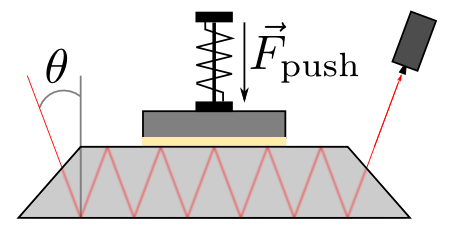
\includegraphics[width=0.8\linewidth]{./figs/IRoverview}
	\caption{}
	\label{fig:iroverview}
\end{subfigure}
\begin{subfigure}{0.5\textwidth}
\centering
	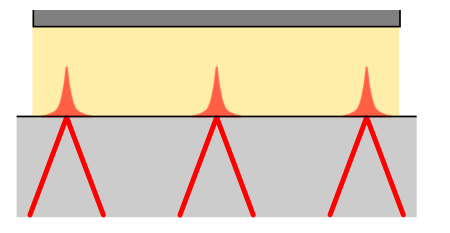
\includegraphics[width=0.8\linewidth]{./figs/IRwave}
	\caption{}
	\label{fig:irwave}
\end{subfigure}
\caption{Schematic of an \atr{} \ftir{} set-up. Figure \ref{fig:iroverview} shows the internal reflection of the beam of light at the edges of the guiding crystal (light gray) and the thin film sample (yellow) on its substrate (dark grey) being pressed onto the crystal. Figure \ref{fig:irwave} focuses on the evanescent wave projecting into the thin film and gives an indication how the beam, while being nominally inside the crystal, can still be attenuated by the sample. Adopted from VILAN.}
\label{fig:irscheme}
\end{figure}
To study thin films that are either physically or chemically adsorbed to a substrate surface, it is useful exclude interaction of the substrate with the \ir{}-radiation and to maximise the interactions interactions that are of interest. One method that accomplishes  both these goals is Attenuated Total Reflectance (\atr{}) \ftir{} where the \ir{} beam is directed into a crystal of high refractive index and reflects internally from its surfaces. Refer to Figure \ref{fig:irscheme} for a schematic of the \atr{} method. The thin film under investigation is pressed onto the crystal to form an intimate contact so that an evanescent \ir{} wave can project into it, see Figure \ref{fig:irwave}. There, part of the \ir{} spectrum is absorbed by the sample and the now somewhat reduces beam is returned into the crystal where it can be internally reflected to be projected into the thin film again multiple times, greatly attenuating the absorption of the thin film. As can be deduced from Figure \ref{fig:iroverview}, the reflectance is given by
\begin{equation}
\label{atr-reflectance}
	R(\lambda)^N = (1-a_{\lambda} \cdot d_e)^N \, ,
\end{equation}
where $N$ is the number of reflections taking place at the crystal/thin film interface~\footnote{For the case of Figure \ref{fig:irscheme} $N=3$}, $a_{\lambda}$ is the wavelength specific absorptivity of the thin film and $d_e$ is its effective thickness. One complication that needs to be mentioned is that \atr{} spectra are not linear with wavenumber CITE VILAN and therefore sometimes difficult to compare to transmittance spectra. In the context of this study, that complication is somewhat alleviated because we will mainly compare \atr{}-\ftir{} spectra relative to other other \atr{}-\ftir{} spectra to assess whether or not a phase transition has occurred in the thin film sample and will for the most part not need absolute quantification of the samples.
\subsection{Ellipsometry and contact profilometry}
\subsubsection{Ellipsometry}
Generally, ellipsometry is an optical technique for investigating the dielectric properties of (layers of) thin films of material(s) on reflective surfaces. It is an indirect method insofar as that the information obtained from an ellipsometry measurement cannot directly be converted into the dielectric properties of the thin film under investigation. Therefore, the measured data must be compared to a model and the success of an ellipsometry measurement hinges on the quality of that model. In its most common form, ellipsometry measures the properties of light reflected from the surface of a sample. The set-up consists of a light source, a polariser, the sample, an analyser and a detector. Light with known, elliptical polarisation is employed, hence the name. This incident light can be decomposed into two components: the \emph{s} component where the electrical field of the radiation oscillates parallel to the sample and perpendicular to the plane of incidence and the \emph{p} component where the field oscillates parallel to the plane of incidence. Ellipsometry measures the complex reflectance $\rho$ of the sample which consists of an amplitude component $\Psi$ and a phase difference $\Delta$ according to
\begin{equation}
	\rho = \tan \left( \Psi \right) \exp \left( i \Delta \right) \, .
\end{equation}
The complex nature of the reflectance as measured by ellipsometry is readily apparent from the equation above. Per wavelength, one pair of $\Psi$ \& $\Delta$ can be obtained. Therefore, to reach more optical parameters, a broad spectrum is often employed in ellipsometry. For the purposes of this study, ellipsometry was exclusively used to find the thickness of a layer of interest on a substrate of known composition and thickness.
\subsubsection{Contact Profilometry}
Contact profilometry is a conceptually exceedingly simple technique to study surfaces and their roughness. A small diamond tip is brought in contact with a surface and moved across a predefined path along that surface and vertical displacement of the stylus is measured accurately. Depending of the type of surface under investigation displacements of \SI{10}{\nano\metre} up to \SI{1}{\micro\metre} can typically be measured with a lateral resolution depending primarily on the size of the tip-apex, where resolutions of $\sim$\SI{20}{\nano\metre} are feasible. The diamond tip of a record player scanning a vinyl record and producing an audible, analogue signal is a very fitting analogy for contact profilometers in use today.
\subsection{Electron Microscopy}
While a thorough explanation of the function and uses of electron microscopy is out of the scope of this paper, a brief introduction to Scanning Electron Microscopy (\sem{}) for the visualisation of nanometre sized objects will still be given. \sem{} is a type of electron microscopy in which a sample is raster-scanned with a focused beam of electrons. This focused beam causes the sample to emit several types of signals: secondary electrons emitted by atoms in the sample, backscattered electrons, x-rays and light of varying wavelength and intensity, all of which can be detected by sophisticated microscopes. The resolution of the microscope is not achieved as in an optical microscope or as in a Transmission Electron Microscope (\tem{}) where the focusing the beam and the wavelength are determining, but rather by a translation of the size of the raster on the sample to the size of the raster on the detector. Thus, \sem{} can cover up to six orders of magnitude of magnification and sample features at very different length scales can be investigated. Because the sample is subjected to a continuous beam of electrons, it needs to be conductive and grounded to get rid off excess charge. Charge accumulated on the sample can lead to unwanted interactions and artefacts in the visual reconstruction of the sample. For the purpose of this study, \sem{} was used to investigate the surface morphology of deposited thin films of a polymer, \pvdf{}, and nanoparticles synthesised from the same polymer. \sem{} was also used to obtain typical nanoparticle dimensions.
\subsection{IV-curves}
Current-Voltage curves (IV-curves) of a semiconductor or solar cell can reveal a lot of information about the semiconductor or cell under investigation, not withstanding its conceptual simplicity. In a straight forward measurement, two contact are electrically connected to the sample and the current resulting from a precisely known applied voltage is measured accurately. With an appropriate illumination set-up, dark and light IV-curves can be obtained and compared. For an ideal diode, the dark current is given by the diode equation:
\begin{equation}
	I = I_0 \left( \exp \left( \frac{qV}{nk_BT} \right) -1 \right) \, ,
\end{equation}
where $I_0$ is the reverse saturation bias current, $n$ is the ideality factor and the remaining symbols have their usual meaning. Under light conditions, a steady-state current is induced that shifts the IV-curve down, depending on the size of the photon-current, their spectrum and the cell's spectral response. A \enhyphen{real} diode will also include parasitic resistances such as series resistance $R_S$ and shunt resistance $R_{SH}$ and the measured IV-curve will more closely follow a form corresponding to the equation:
\begin{equation}
	I = I_0 \left( \exp \left( \frac{q(V+IR_S)}{nk_BT} \right) -\frac{V+IR_S}{R_{SH}} \right) \, .
\end{equation}
As can be seen from the above equation, the parasitic resistances can be obtained from the derivative of of the IV-curve at its intersections with the axes and to put it more colloquially, parasitic resistances will result in the IV-curve being \enhyphen{less square} than than of its ideal counterpart. The presence of back-diodes will result in a \emph{S}-shaped or otherwise generally misshapen IV-curves and while it is often useful to extract precise cell parameters such as fill-factor, open-circuit voltage and short-circuit current, optical inspection of the IV-curve alone may already reveal key issues with a cell under investigation.
\subsection{Dynamic Light Scattering}
\begin{figure}
\begin{subfigure}{0.5\textwidth}
\centering
	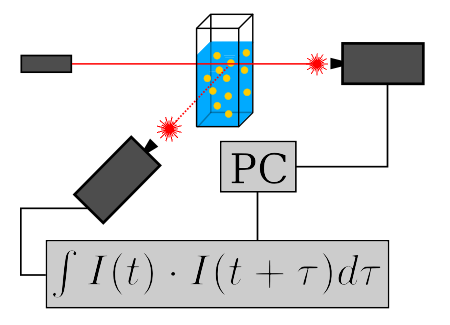
\includegraphics[width=0.8\linewidth]{./figs/dlssetup}
	\caption{}
	\label{fig:dlssetup}
\end{subfigure}
\begin{subfigure}{0.5\textwidth}
\centering
	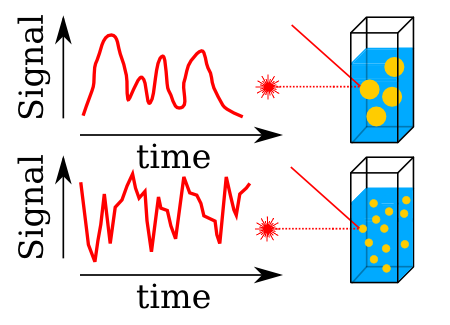
\includegraphics[width=0.8\linewidth]{./figs/dlsnoise}
	\caption{}
	\label{fig:dlsnoise}
\end{subfigure}
\caption{A schematic of a typical, simplified \dls{} set-up. Figure \ref{fig:dlssetup} shows the main components: (laser) source, sample cell, detectors, auto-correlator and a computer for data-sampling. Two detectors allow for measurement of relative intensity and thus help reduce unwanted noise from fluctuations in laser intensity. Figure \ref{fig:dlsnoise} shows how different particle sizes lead to different \enhyphen{noise} signatures in the measured signal.}
\label{fig:dlscheme}
\end{figure}
Dynamic Light Scattering (\dls{}) is most commonly used to analyse nanoparticles, specifically it can be used to determine the size of nanoparticles in solution. The optical set-up of a \dls{} experiment is shown in Figure \ref{fig:dlssetup}, a typical example of the the obtained optical signal is shown in Figure \ref{fig:dlsnoise}. A laser illuminates the sample, some amount of light is scattered by particles in solution and its intensity as a function of time is determined by the detector at an angle to the path of the laser beam. A second detector in the direct path of the light is used to subtract fluctuations in laser intensity. The \enhyphen{noise} in the measured relative intensity of the two detectors is a direct consequence of the (Brownian) motion of nanoparticles in solution and will be used to extract particle size. As particles move into and out of the path of the laser, more or less light will be scattered toward the detector. Furthermore, a particle that moves about but stays within the path of the beam for a certain delay time $\tau$ will continue to scatter light. Therefore, the evolution of the \enhyphen{noise} in time can be understood in terms of an autocorrelation function. The mathematical treatment of the signal from a population of nanoparticles with different sizes is complicated and mathematically ill posed. To overcome this difficulty experimentally, restrictions on the size distribution have to be supplied. The following discussion will be restricted to a nanoparticle population of a single size so as not to exceed the scope of this project. For such a population, the autocorrelation function
\begin{equation}
	C(\tau) = \sum _{t=0}^T I(t)\cdot I(t + \tau) \, ,
\end{equation}
where $T$ is the total time of the experiment, $I(t)$ is the intensity at time $t$ and $I(t + \tau)$ is the intensity at time $t+\tau$, will also be given by a simple exponential decay:
\begin{equation}
	C(\tau) = \exp (-2 \Gamma \tau) + B \, ,
\end{equation}
where $B$ is a baseline intensity and where $\Gamma$ is obtained by a data-fit and is related to the (translational) diffusion coefficient $D_t$ by the scattering vector $q$ as:
\begin{equation}
	\Gamma = D_t \cdot q^2 = D_t \left( \frac{4 \pi n}{\lambda} \sin \left( \frac{\theta}{2} \right) \right) ^2 \, .
\end{equation}
In the last equation $n$ is the refractive index of the medium, $\lambda$ is the wavelength of scattered light and $\theta$ is the scattering angle. Finally, $D_t$ as determined from the data-fit can be used in the Stokes-Einstein relation for Brownian motion to find the apparent hydrodynamic diameter $D_h$ of the suspended particles:
\begin{equation}
\label{diameter}
	D_h = \frac{k_B T}{3\pi \eta D_t} \, .
\end{equation}
Here, $k_B$ is the Boltzmann constant, $T$ is the thermodynamic temperature and $\eta$ is the viscosity of the suspending medium. As can easily be seen in Equation \eqref{diameter}, the determined particle diameter is directly proportional to the absolute temperature $T$, however, the viscosity of the medium is usually also very sensitively dependent on temperature and a specific value for $\eta$ needs to be supplied for the measurement. For practical purposes, the viscosity of typical (mixtures of) solvents in a range of temperatures is internally tabulated by software, as are their refractive indices. Therefore, the user of a \dls{} apparatus supplies the type of solvent used, the machine monitors the temperature during the experiment and carries out the necessary calculations and data-fitting routines. It is important to note that, for a successful size determination via \dls{}, a solution of nanoparticles should be sufficiently dilute to avoid clusters of nanoparticles while at the same time being concentrated enough to allow for measurable scattering intensities. Furthermore, the Stokes-Einstein relation assumes rigid, spherical particles so the apparent diameter of a soft, ovoid particle may significantly differ from its true dimensions.

\section{Experimental Approach \& Results}
\label{sec:expwork}
\subsection{Sample Prep}
\subsubsection{Si-H}
\subsubsection{Nanoparticles}
\subsection{\pvdf{} poling, annealing}
\subsection{CPD SPV}
\subsubsection{Standard Experiments}
\subsubsection{Pole-Reverse-Pole}
\subsection{Lifetimes}
\subsection{Ellipsometry}
\subsection{\ir{}}
\subsection{IV}
\subsection{Microscopy}
\subsection{\dls{}}


\section{Discussion}